\documentclass[12pt,a4paper]{report}

%-------------------------------------------------
%   PACKAGES & CUSTOMIZATION
%-------------------------------------------------
\usepackage[utf8]{inputenc}
\usepackage[T1]{fontenc}
\usepackage{lmodern}               % Modern Latin font
\usepackage[english]{babel}
\usepackage[margin=1in]{geometry}  % Adjust margins
\usepackage{setspace}              % For line spacing
\usepackage{amsmath,amssymb}       % Math packages
\usepackage{graphicx}              % For including figures
\usepackage{booktabs}              % For professional-quality tables
\usepackage{hyperref}              % Hyperlinks in PDF
\usepackage{caption}               % Improved captions
\usepackage{subcaption}            % Subfigures
\usepackage{enumitem}              % Better list environments
\usepackage{float}
\usepackage{listings}

% Optional: Bibliography package if needed
%\usepackage[backend=biber,style=apa]{biblatex}
%\addbibresource{references.bib}

% One-and-a-half line spacing
%\onehalfspacing

%-------------------------------------------------
%   TITLE PAGE INFORMATION
%-------------------------------------------------
\title{RoadSense: Healthier Roads, Safer Journeys \\ \vspace{0.5em}
\Large Edge Computing in the IoT \\ Università della Svizzera italiana (USI)}

\author{Luca Di Bello, Paolo Deidda, Nawfal Abdul Malick, Georg Meyer \\[1em]
Semester Project}

\date{Due: 20 December 2024}

%-------------------------------------------------
%   BEGIN DOCUMENT
%-------------------------------------------------
\begin{document}

\maketitle

\tableofcontents
\listoffigures

%-------------------------------------------------
%   CHAPTER 1: System Design
%-------------------------------------------------
\chapter{System Design}
\section{Introduction}

The \textbf{RoadSense} project seeks to develop an IoT-powered system for detecting and mapping road anomalies, such as potholes and uneven surfaces. By equipping multiple vehicles with sensor nodes, the system will gather and analyze road vibration data to generate an interactive, detailed heatmap of road conditions. This data will be instrumental in optimizing road maintenance, enhancing driver safety, and providing real-time hazard alerts.

The project aims to deliver a comprehensive solution for road condition monitoring by addressing key objectives across data collection, processing, visualization, and alerting. Specifically, the system will focus on:

\begin{enumerate}[label=\arabic*.]
	\item Designing a cost-effective IoT-based solution for detecting and mapping road anomalies.
	\item Measuring road bumpiness and issuing real-time alerts for hazardous conditions.
	\item Providing a user-friendly interface for stakeholders to visualize road conditions and manage alerts effectively.
	\item Enhancing road condition accuracy through data collection from multiple vehicles.
\end{enumerate}

\section{Overview}

The \textbf{RoadSense} system consists of the following components:

he \textbf{RoadSense} system consists of the following components:

\begin{itemize}
    \item \textbf{Sensor Nodes}: IoT devices installed in vehicles, responsible for collecting inertial data using an Inertial Measurement Unit (IMU) sensor and location data via a GPS module. These nodes should already compute a qualifier for localized road states to minimize data traffic to centralized hubs.
    \item \textbf{Server-Side Application}: Collects, aggregates, and analyzes data from multiple devices, and visualizes road quality using heatmaps.
    \item \textbf{Control Logic}: Defines the behavior of the IoT device in terms of data collection, processing, and communication.
    \item \textbf{User Interface}: An interactive web application allowing stakeholders to visualize road conditions and manage alerts.
\end{itemize}
\section{Sensor Nodes}

\begin{figure}[ht!]
   \centering
   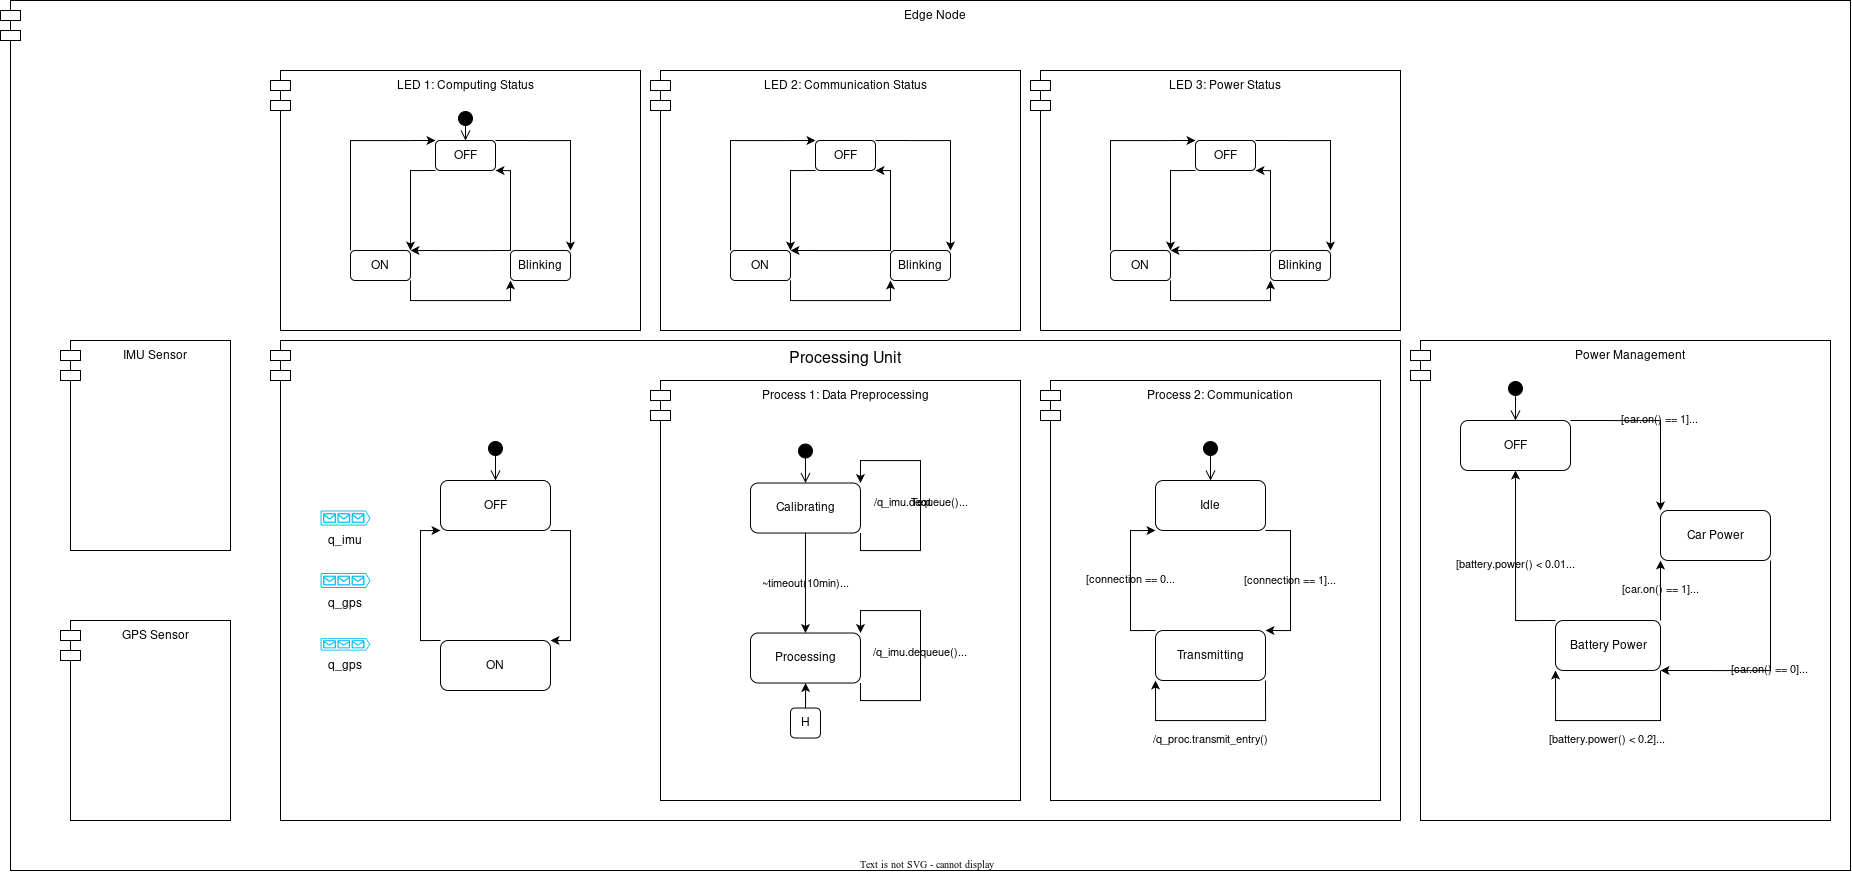
\includegraphics[width=\textwidth]{../../assets/diagrams/edge_node_rtuml/edge_node_rtuml.png}
   \hfill
   \caption{RT-UML of a Sensor Node}
   \label{fig:rt_uml_sensor_node}
\end{figure}

\begin{enumerate}
    \item \textbf{Cost Restriction per Node}: ~100 CHF \\
        Given the large number of vehicles that will host sensor nodes, the cost per node must remain as low as possible. To achieve this, each vehicle will have a single sensor node/package installed to minimize installation and part costs.

    \item \textbf{Quantification of Road State}: \\
        The sensor node will be ideally positioned centrally in the vehicle, above one of the axles, and securely mounted to the chassis to reduce measurement errors. The road state will be quantified on a scale from 0 (very good) to 244 (very poor), with 255 reserved for hazardous conditions.

    \item \textbf{Adaptation of Quantification to Vehicle Types and Driving Conditions}: \\
        A simple linear Mass-Spring-Damper model will be employed to account for the vehicle's influence on shock measurements while maintaining computational efficiency. An initial calibration phase, supported by default parameter settings, will adjust the model to fit the specific vehicle. During calibration, measured data will be mapped to quantified road state values. Additionally, other physical quantities beyond z-axis acceleration will be incorporated to decouple road state data from driving-induced accelerations.

    \item \textbf{High Polling Rate for IMU Measurements}: \\
        Road-induced shocks are brief and their period and amplitude are proportional to vehicle speed. The IMU's polling rate will be configured to ensure reliable readings for typical driving speeds.

    \item \textbf{Sensing of Physical Quantities}: \\
        The system will measure multiple physical quantities to ensure accurate road state assessments:
        \begin{enumerate}
            \item \textbf{Z-Axis Acceleration}: For detecting road conditions and potholes. Polling rate must adapt to vehicle velocity and be sufficiently high.
            \item \textbf{X- and Y-Axis Acceleration and Rotational Acceleration}: To minimize errors caused by driving dynamics.
            \item \textbf{Driving Velocity}: To correlate shock amplitudes with velocity using the Mass-Spring-Damper model.
            \item \textbf{Geographical Position}: To map road state measurements to specific locations.
        \end{enumerate}

    \item \textbf{Data Transmission at Established Gatepoints}: \\
        \begin{enumerate}
            \item \textbf{Data Format}: Each data package will include the following information encoded as a JSON object:
              \begin{lstlisting}[breaklines=true, basicstyle=\ttfamily]
(Node ID (2 Bytes)) | Position (2 x 8 Bytes (Double-Precision Float)) | Road Quality (1 Byte) | Unix Timestamp (4 Bytes)
              \end{lstlisting}

              For example, the following snippet represents a valid data sample in JSON format:

              \begin{lstlisting}[breaklines=true, basicstyle=\ttfamily]
{               
  "lat": 46.19313,
  "lon": 6.80421,
  "timestamp": 1734478933,
  "bumpiness": 50,
  "device_id": "USI-Car-1""
}
              \end{lstlisting}

            \item \textbf{Local Preprocessing}: The node will preprocess and store position-quality tuples locally.
            \item \textbf{Gatepoint Connectivity}: The node will automatically establish a connection at predefined gatepoints to transmit new data.
            \item \textbf{Data Protocol}: Data packages will be transmitted in MQTT format to a RabbitMQ server.
        \end{enumerate}
\end{enumerate}

\section{System Architecture}

The \textbf{RoadSense} consists of multiple IoT devices installed in vehicles, communicating with a central server designed to be highly scalable to handle data from thousands of devices. In this section we will describe all meaningful components of the system, focusing on the IoT data pipeline and the client-server architecture.

\subsection{IoT Data Pipeline}
\label{subsec:iot_data_pipeline}

The data pipeline has been designed with scalability in mind, allowing for efficient data collection, processing, and data analysis from multiple (potentially thousands) concurrent IoT devices. The following diagram illustrates the pipeline steps, from data ingestion to the storage of processed data.

\begin{figure}[H]
	\centering
	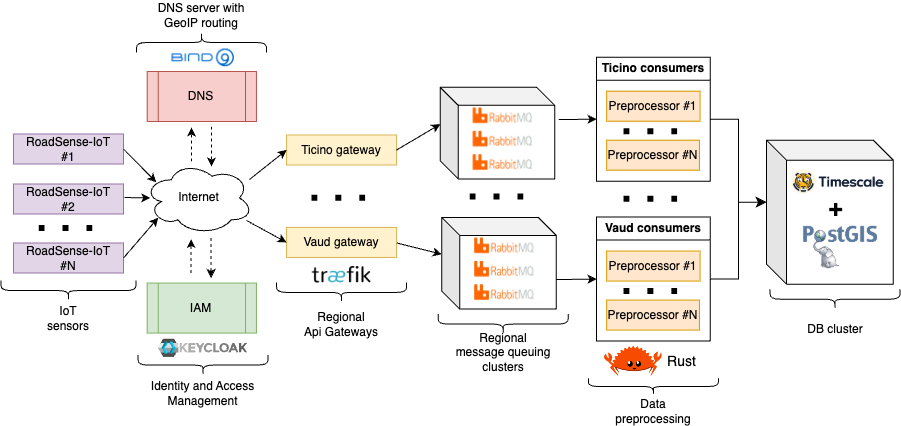
\includegraphics[width=\textwidth]{../../assets/diagrams/iot_data_pipeline/iot_data_pipeline.png}
	\caption{IoT Data Pipeline}
\end{figure}

The pipeline consists of the following components:

\begin{enumerate}
	\item \textbf{Data ingestion}: IoT devices collect vibration, GPS, and other relevant data points. When the vehicle reaches an access point, the data will be transmitted to the server. Each device will be able to connect to different Wi-Fi networks, allowing for data transmission in different locations. This may include public Wi-Fi networks, cellular data, or a dedicated network infrastructure.

	\item \textbf{Authentication and security}: In the original idea of the project each device is authenticated before data transmission to ensure data integrity and prevent unauthorized access. For this purpose, was decided to use \href{https://www.keycloak.org/}{Keycloak} for identity and access management. Unfortunately, this feature was not implemented in the presented prototype in order to focus on the core functionality of the system.

	\item \textbf{Geographical distribution}: The server leverages DNS-based load balancing to distribute incoming data across regional gateways for efficient processing. We have chosen to use \href{https://www.isc.org/bind/}{BIND9} for DNS-based load balancing along with \href{https://www.maxmind.com/en/geoip2-databases}{GeoIP} for geolocation. Each regional gateway will be responsible for routing the user requests to the regional message queuing system. For this purpose, we will use \href{https://traefik.io/}{Traefik} as the reverse proxy. Unfortunately, also this feature was not implemented in the prototype as it would introduce additional complexity to the system. However, this feature is essential for the scalability of the system as it allows for efficient data processing across multiple regions.

	\item \textbf{Message queues}: Each gateway node processes incoming data and forwards it to a regional queuing system to allow for parallel processing. After evaluating multiple options, we decided to use \href{https://www.rabbitmq.com/}{RabbitMQ} as the message queue system. To ensure high availability, we will deploy RabbitMQ in a cluster configuration (refer to the \href{https://www.rabbitmq.com/clustering.html}{RabbitMQ Clustering Guide}). For the prototype we avoided the creation of a RabbitMQ cluster, and was used a single instance of RabbitMQ. This feature is still of interest for the scalability of the system.

	\item \textbf{Data preprocessing}: Each region has a set of preprocessing microservices that consume incoming data from the regional message queuing system, perform data validation, and run initial data processing tasks. These microservices are deployed using containerization technology like Docker and in a future production environment, managed by \href{https://kubernetes.io/}{Kubernetes}.
	      During the initial specification of the project was decided to use \href{https://golang.org/}{Go} as the primary language for these microservices. However, in the prototype was used \href{https://rust-lang.org/}{Rust} as the primary language for the microservices. This choice was made to explore the performance and safety features of Rust. The microservices were designed to be lightweight, efficient and fail-safe.

	\item \textbf{Data storage}: Processed data is stored in a scalable database system that can handle high volumes of data. Since we are dealing with both date-time and geospatial data, we chose to use \href{https://www.timescale.com/}{TimescaleDB} as the database system with the \href{https://postgis.net/}{PostGIS} extension to support geospatial queries.
	      PostGIS was used to store and query collected samples
\end{enumerate}

\subsection{Client-Server interaction}

The \textbf{RoadSense} system employs a client-server architecture designed to efficiently deliver real-time road condition data. The client is a web-based application that visualizes road condition samples on an interactive map. These samples are fetched from a custom API microservice, which only returns data points within the map's current bounding box, leveraging \textbf{PostGIS} for spatial queries to optimize performance and minimize data transfer. This ensures scalability and efficient handling of large datasets, as the system can support millions of samples without overwhelming either the client or the server. The following diagram illustrates the client-server interaction:

\begin{figure}[H]
	\centering
	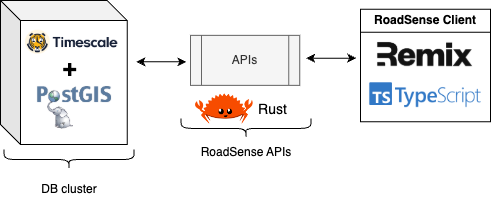
\includegraphics[width=\textwidth]{../../assets/diagrams/client_server_architecture/client_server_arch.png}
	\caption{Client-Server Interaction}
\end{figure}

\noindent The backend is implemented as a custom API server built with \textbf{Rust} using the \textbf{Actix} web framework and \href{https://diesel.rs/}{Diesel} for database interaction. It provides a read-only interface, returning road condition samples in \texttt{JSON} format based on client requests. Data insertion is handled by separate consumers processing messages from \textbf{RabbitMQ}. The architecture enables efficient data processing, retrieval, and real-time visualization while maintaining scalability and performance.


%-------------------------------------------------
%   CHAPTER 2: Description of system implementation
%-------------------------------------------------
\chapter{System Implementation}

\section{Overview}

The \textbf{RoadSense} system consists of the following components:

he \textbf{RoadSense} system consists of the following components:

\begin{itemize}
    \item \textbf{Sensor Nodes}: IoT devices installed in vehicles, responsible for collecting inertial data using an Inertial Measurement Unit (IMU) sensor and location data via a GPS module. These nodes should already compute a qualifier for localized road states to minimize data traffic to centralized hubs.
    \item \textbf{Server-Side Application}: Collects, aggregates, and analyzes data from multiple devices, and visualizes road quality using heatmaps.
    \item \textbf{Control Logic}: Defines the behavior of the IoT device in terms of data collection, processing, and communication.
    \item \textbf{User Interface}: An interactive web application allowing stakeholders to visualize road conditions and manage alerts.
\end{itemize}
\section{Prototype Car}

\begin{figure}[ht!]
    \centering
    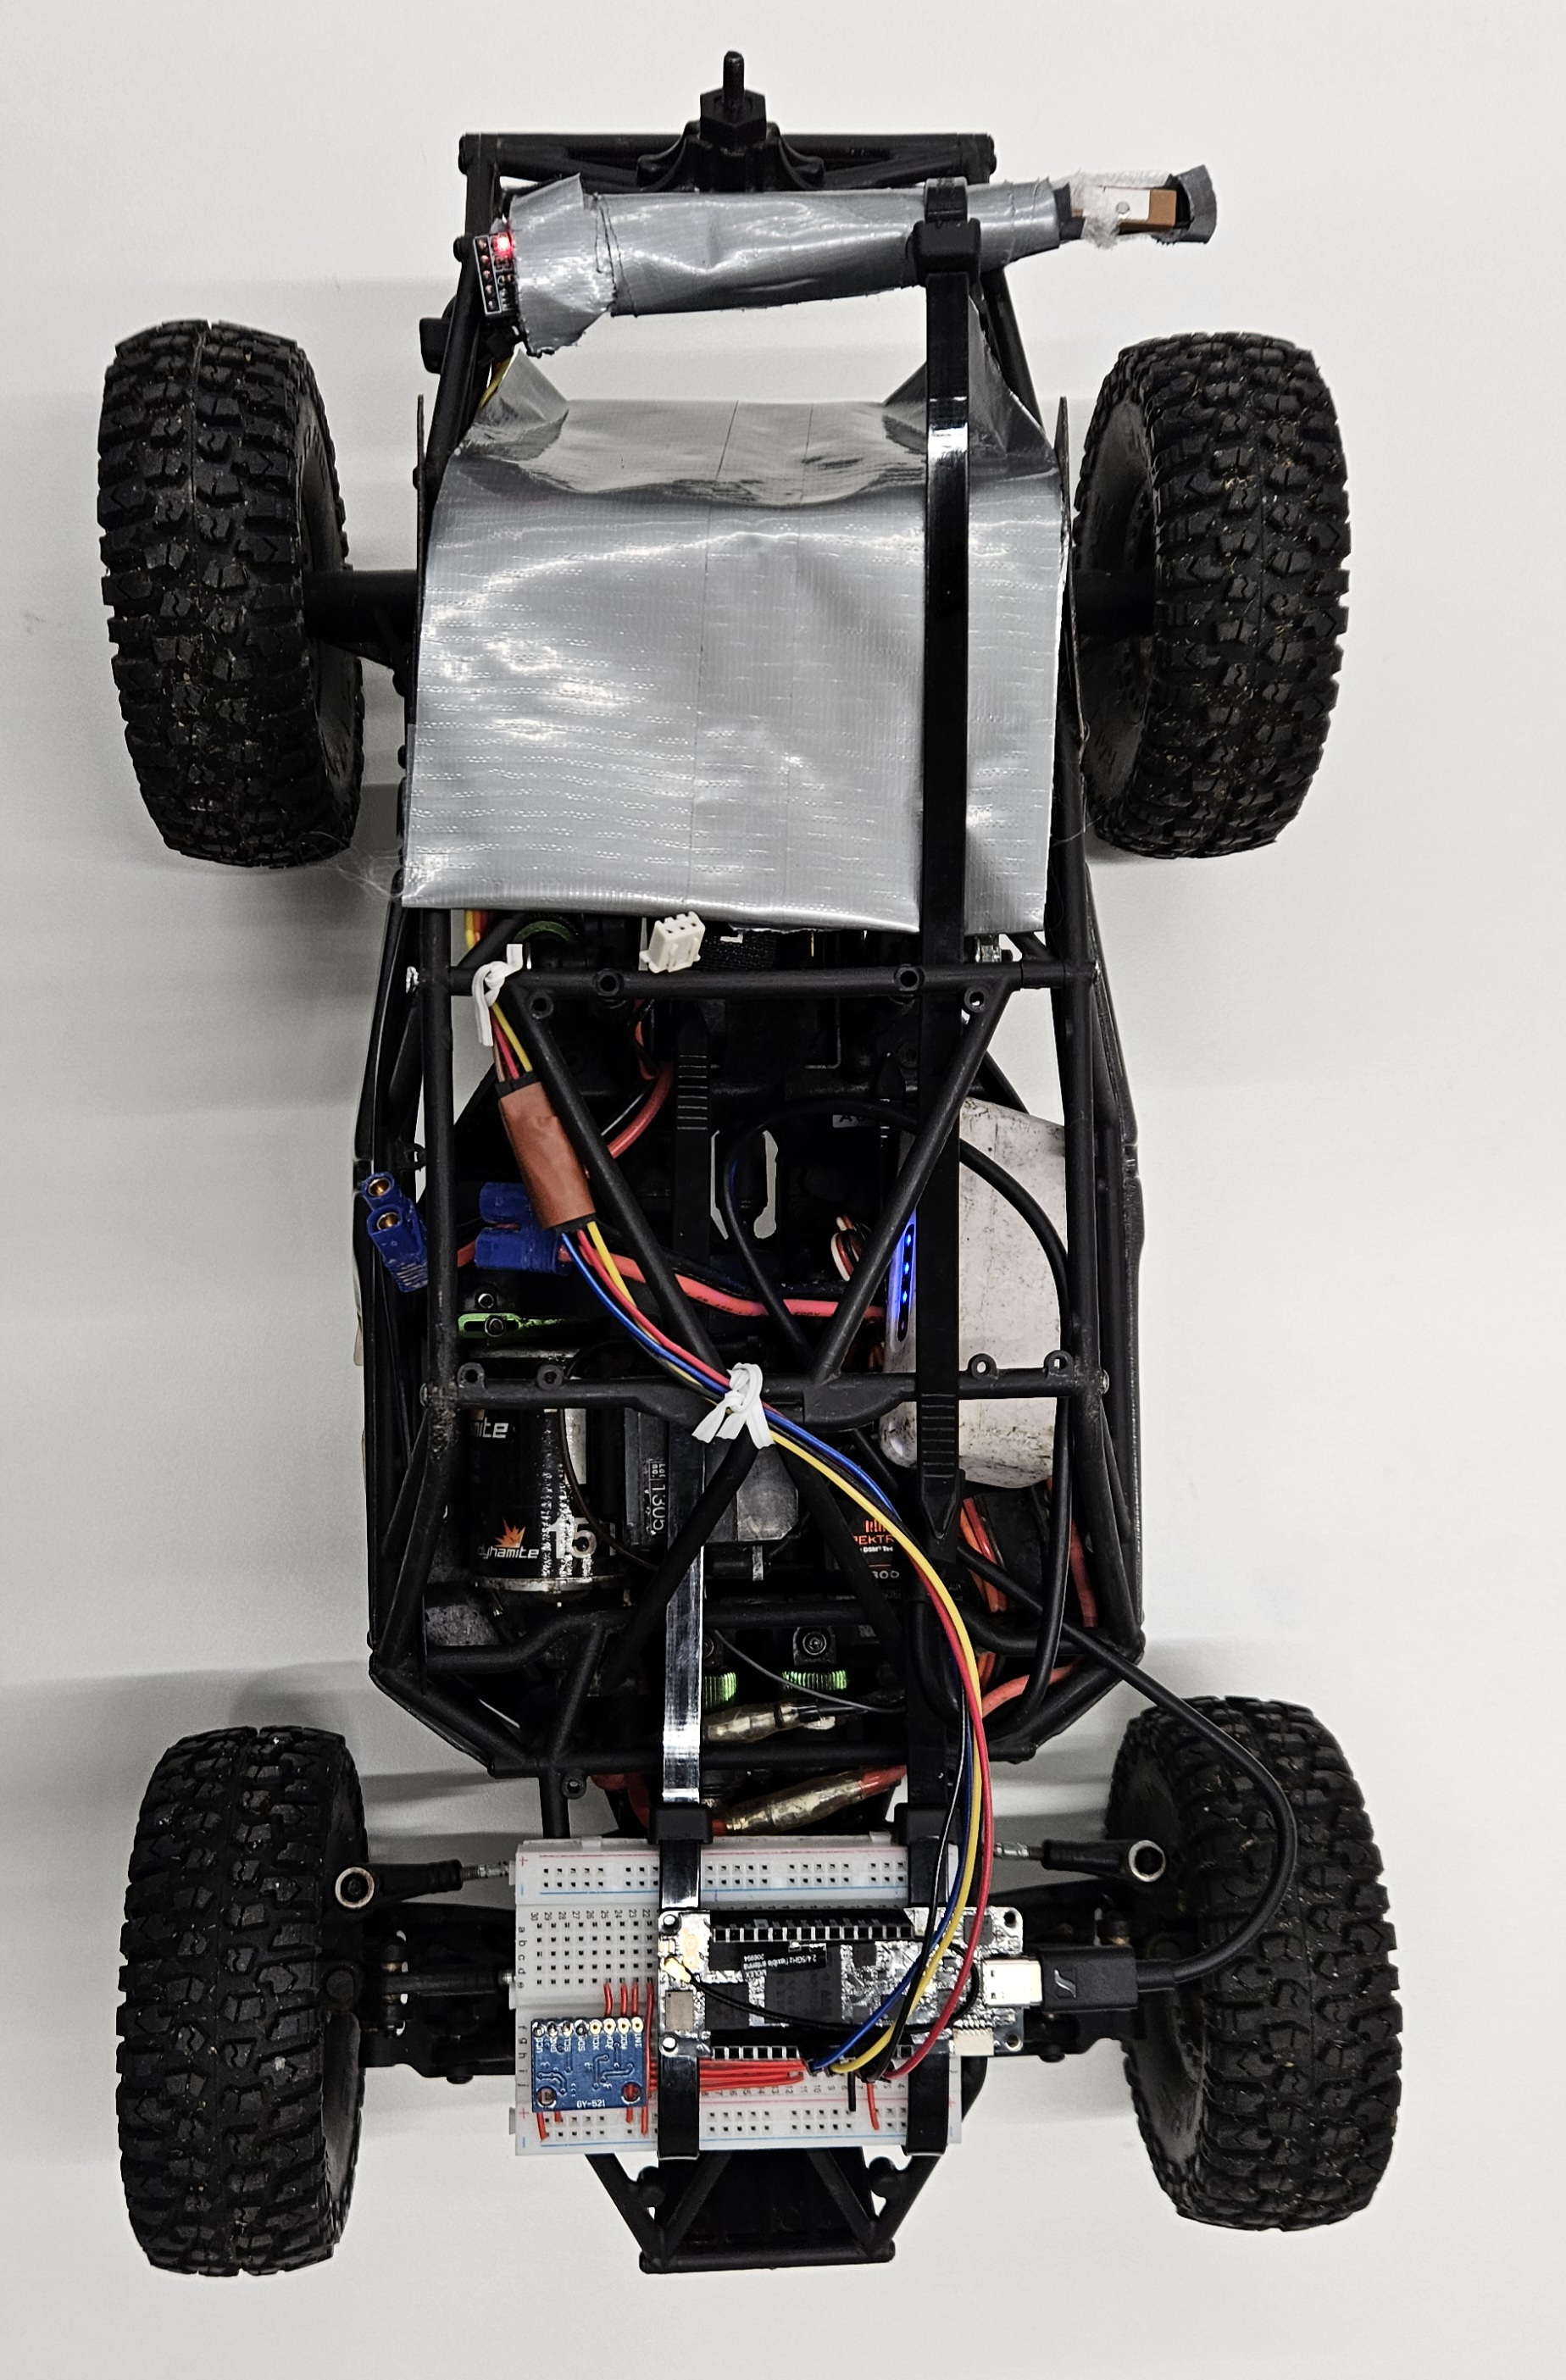
\includegraphics[angle=90,width=0.7\textwidth]{../../assets/images/roadsense_rc_top.jpg}
    \caption{RoadSense Prototype RC Top View}
\end{figure}

\subsubsection{Hardware Components}

\begin{enumerate}
    \item \textbf{Microcontroller}: \\
        \textbf{Arduino Portenta H7} with built-in Wi-Fi capability and RTOS support. \\
        Enables usage of threads for sensor data collection and transmission.
    \item \textbf{IMU Sensor}: \\
        \textbf{GY-521} with MPU6050 6DOF (3-Axis Gyro and 3-Axis Accelerometer). \\
        While currently only the z-axis acceleration is used, the sensor provides additional data which can be used for future work to improve the road state qualification model.
    \item \textbf{GPS Module}: \\
        \textbf{DFRobot GPS + BDS BeiDou} with output of position and speed. \\
        We were able to fix connectivity by integrating EMF shielding. As the transmitted speed data was faulty, we had to make use of a fallback solution by approximating each segment through a fixed time of 3 seconds.
    \item \textbf{EMF Shielding}: \\
        \textbf{DIY} using aluminum foil to shield the GPS module from electromagnetic interference.

\end{enumerate}

Detailed information on the pin connections for the sensors with the Arduino Portenta H7 can be found in Table \ref{tab:sensor_connections}.

\begin{table}[h!]
    \centering
    \begin{tabular}{|l|l|l|p{8cm}|}
    \hline
    \textbf{}         & \textbf{Sensor}       & \textbf{Portenta H7}            & \textbf{Description}                                                    \\ \hline
    \textbf{GY-521}         & VCC                   & 3.3V                            & Power supply (3.3V)                                                     \\ \cline{2-4}
                            & GND                   & GND                             & Ground                                                                  \\ \cline{2-4}
                            & SDA                   & SDA (Pin 11)                    & I2C Data line (SDA)                                                     \\ \cline{2-4}
                            & SCL                   & SCL (Pin 12)                    & I2C Clock line (SCL)                                                    \\ \hline
    \textbf{DFRobot GPS}    & VCC                   & 3.3V                            & Power supply (3.3V)                                                     \\ \cline{2-4}
                            & GND                   & GND                             & Ground                                                                  \\ \cline{2-4}
                            & TX                    & RX (Pin 13)                     & Serial data transmit line \newline (TX from GPS to RX on Portenta H7)   \\ \cline{2-4}
                            & RX                    & TX (Pin 14)                     & Serial data receive line \newline (RX from GPS to TX on Portenta H7)    \\ \hline
    \end{tabular}
    \caption{Pin Connections for Sensors with Arduino Portenta H7}
    \label{tab:sensor_connections}
    \end{table}
\section{Prototype Embedded Firmware}

In this section, we provide an overview of the core components and implementation details of the prototype embedded firmware developed for the sensor node. The firmware orchestrates sensor data acquisition, road quality analysis, and reliable data transmission to an external system.
The following subsections summarize the primary files and their responsibilities:

\begin{itemize}
    \item \textbf{Mainfile (roadsense-embedded.ino):} Initializes the system, sets up multithreaded operations, and manages the data flow between sensor acquisition and network transmission.
    \item \textbf{roadqualifier.h:} Contains the logic for measuring, calibrating, and quantifying road segment quality using integrated sensors, along with persistent calibration data handling.
    \item \textbf{RabbitMQClient.h:} Handles WiFi connectivity and MQTT-based communication, enabling the sending of computed road quality metrics to a RabbitMQ server.
\end{itemize}

By clearly defining these components, the firmware maintains a modular structure, simplifying development, testing, and future enhancements.

\subsection{Mainfile (roadsense-embedded.ino)}

The main Arduino \texttt{roadsense-embedded.ino} file serves as the central entry point for the embedded firmware running on the sensor node. Its primary tasks involve initializing system components, orchestrating two concurrent threads for road data acquisition and transmission, and managing communication buffers.

\begin{itemize}
    \item \textbf{Initialization and Setup:}  
    At startup, the main file initializes serial communication for debugging. It then sets up the \texttt{RoadQualifier} instance, which prepares sensor input (e.g., IMU and GPS readings) for analyzing road quality. If initialization fails, the system reports this via serial output.

    \item \textbf{Multithreading using Mbed OS:}  
    Leveraging Mbed OS RTOS features, the firmware runs two threads concurrently:
    \begin{enumerate}
        \item \textit{Road Segmentation Thread}: Periodically calls \texttt{roadQualifier.qualifySegment()} to compute the quality of a road segment. Upon success, it stores the resulting \texttt{SegmentQuality} record into a thread-safe circular buffer.
        \item \textit{Data Transmission Thread}: Establishes and maintains a WiFi connection, then continuously reads from the circular buffer to transmit data using a \texttt{RabbitMQClient}. If no data is available, it waits until new records arrive.
    \end{enumerate}

    \item \textbf{Circular Buffer for Data Storage:}  \\
    A custom circular buffer, protected by a mutex, ensures safe concurrent access from both threads. If the buffer is full, the oldest entry is overwritten, preventing blocking conditions and ensuring efficient memory usage.

    \item \textbf{Data Transmission via RabbitMQ:}  \\
    Once connected to WiFi, the data transmission thread publishes buffered \texttt{SegmentQuality} records to an external system through the \texttt{rabbitMQClient}. This design decouples data acquisition from network-related issues, allowing both to operate independently.

    \item \textbf{Watchdog and Timing:}  \\
    Although not fully explored in the provided snippet, the code includes a watchdog timer and uses \texttt{ThisThread::sleep\_for()} to handle timing and maintain system responsiveness.

    \item \textbf{Main Loop:}  \\
    The \texttt{loop()} function remains empty, as the system relies on RTOS threads for ongoing tasks. All main logic thus resides in separate threads defined in the setup phase.
\end{itemize}

\subsection{roadqualifier.h}

The \texttt{roadqualifier.h} file encapsulates the logic and data structures required to process road quality measurements from connected sensors, manage calibration and data persistence, and ensure system readiness. This file defines the \texttt{RoadQualifier} class, which serves as the core of the road quality analysis functionality.

\begin{itemize}
    \item \textbf{Sensor Abstraction and Dummy Modes:}  
    The code supports both actual hardware operation and dummy sensor modes for testing without physical IMU or GPS devices. Conditional compilation flags (e.g., \texttt{DUMMY\_MPU} and \texttt{DUMMY\_GPS}) select between real and simulated sensor inputs. This approach allows for development and debugging of other modules without actual available sensors.

    \item \textbf{Road Segment Qualification:}  
    The \texttt{RoadQualifier} class provides a \texttt{qualifySegment()} method to measure a predefined road segment’s quality. It uses acceleration data (from the MPU6050 or dummy equivalent) and position/speed data (from a GPS module or dummy object) to compute a \texttt{SegmentQuality} metric. If a valid segment is detected, it returns a quantized quality value mapped into a byte range.

    \item \textbf{Calibration Handling and Flash Memory:}  
    The file includes routines for:
    \begin{itemize}
        \item \textit{Calibration}: Acquiring accelerometer data over a specified timeframe to determine minimum and maximum values, ensuring that subsequent measurements are interpreted correctly.
        \item \textit{Persistent Storage}: Using Mbed’s \texttt{FlashIAPBlockDevice} and related helpers (\texttt{FlashIAPLimits.h}) to store and retrieve calibration parameters (e.g., minimum and maximum acceleration differences) in non-volatile flash memory.
        \item \textit{Deletion of Calibration Data}: Providing a function \texttt{deleteCalibrationFromFlash()} to erase previously stored calibration information, enabling reset or re-calibration scenarios.
    \end{itemize}

    \item \textbf{Quantification and Mapping:}  
    A dedicated \texttt{quantifyToByte()} function maps computed acceleration differences into a 0–255 byte range based on the caputred calibration data. This allows for easy interpretation, efficient storage and transmission of road quality metrics.

    \item \textbf{Initial Setup and Readiness Checks:}  
    The \texttt{begin()} method initializes sensors, loads or creates calibration data, and ensures a stable GPS fix before considering the system ready. The \texttt{isReady()} method provides a quick way to confirm that the \texttt{RoadQualifier} is fully operational.

    \item \textbf{GPS and IMU Integration:}  
    Functions such as \texttt{waitForValidLocation()} and \texttt{waitForValidSpeed()} ensure that the system obtains reliable, fresh data from the GPS before proceeding. The IMU (or dummy MPU) data is read at each iteration, feeding the computation that identifies peak acceleration differences along the measured road segment.
\end{itemize}

%In summary, \texttt{roadqualifier.h} defines a comprehensive solution for segment-based road quality analysis, integrating calibration, sensor data handling, quantization, and persistent storage management. This modular design allows flexible testing, easy recalibration, and robust operation under real-world conditions.

\subsection{RabbitMQClient.h}

The \texttt{RabbitMQClient.h} file manages the communication between the sensor node and an external RabbitMQ server over MQTT. It encapsulates WiFi connectivity handling, MQTT client operations, and the formatting and publishing of road segment data into a consistent interface.

\begin{itemize}
    \item \textbf{WiFi Connectivity Management:}  
    The class attempts to connect to one of several predefined WiFi networks. It continually checks WiFi status and provides a method \texttt{isConnectedWiFi()} to confirm a successful connection. By iterating through a list of credentials, the code increases the likelihood of establishing a network connection in various deployment environments.

    \item \textbf{MQTT Integration for RabbitMQ:}  
    The \texttt{RabbitMQClient} uses the \texttt{PubSubClient} library to communicate over the MQTT protocol. It sets up the MQTT server (RabbitMQ host, port, user, and password) and ensures a persistent connection. The \texttt{connect()} method and the internal \texttt{ensureConnected()} helper function handle reconnection logic and error reporting.

    \item \textbf{Error Handling:}  
    In case of connection failures or publishing errors, the class stores the MQTT state code, accessible via \texttt{getErrorCode()}. This mechanism aids in debugging and understanding the cause of communication issues.

    \item \textbf{Publishing Data and Callbacks:}  
    To send road segment quality data, the class provides:
    \begin{itemize}
        \item \textit{\texttt{publishSegmentQuality()}}: Converts a \texttt{SegmentQuality} struct into a JSON-formatted message and publishes it to a designated MQTT topic.
        \item \textit{\texttt{sendDataCallback()}}: A method suitable for periodic or callback-driven operations, connecting to the RabbitMQ server (if not connected) and publishing freshly acquired segment data.
    \end{itemize}

    \item \textbf{Integration with the Firmware:}  
    By abstracting away the details of WiFi and MQTT connections, \texttt{RabbitMQClient} allows other parts of the firmware—such as the road qualifier threads—to focus solely on data acquisition and retrieval. The communication logic remains modular, enabling future changes to the network stack or message format without altering the core road quality logic.

\end{itemize}

%In summary, \texttt{RabbitMQClient.h} provides a streamlined interface for connecting to WiFi and reliably sending computed segment quality metrics to an external RabbitMQ server via MQTT. This modular approach ensures that network and communication complexities are well-separated from the sensor data processing logic.
\section{Prototype data processing pipeline}

The prototype implementation of the data processing pipeline is a simplified version of the architecture described in \autoref{subsec:iot_data_pipeline}. Certain components such as \textbf{Keycloak} for authentication, geographical-based routing, and running services in a cluster have been omitted. These decisions were made to streamline development and focus on the core functionality of the system, deferring concerns like scalability and advanced security to future iterations.

The core concept remains consistent with the original design: a \textbf{queuing server} is placed behind a \textbf{reverse proxy} (using \textbf{Traefik}) to provide enhanced security and additional features such as load balancing and request routing. A \textbf{consumer} service then pulls data from the queue, performs preprocessing, and stores the processed data in a database. This approach enables modularity and ensures the data is prepared for subsequent analysis and visualization.

While the current implementation lacks certain advanced features, it retains the essential components to validate the core functionality. This includes the ability to handle incoming IoT data, preprocess it, and store it in a format optimized for the system’s use cases. The pipeline serves as a foundation for future iterations, where scalability, geographical routing, and authentication mechanisms can be incorporated.

\begin{figure}[H]
	\begin{center}
		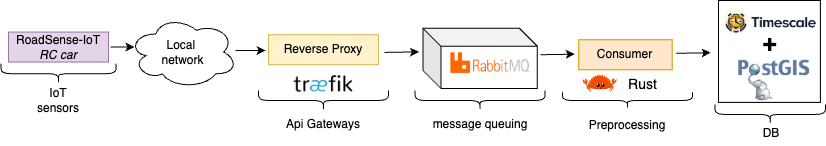
\includegraphics[width=0.95\textwidth]{../../assets/diagrams/prototype_pipeline/prototype_pipeline.png}
	\end{center}
	\caption{Prototype Data Processing Pipeline Architecture}
	\label{fig:prototype_pipeline}
\end{figure}

\noindent This simplified implementation allows for faster prototyping and development while maintaining a clear path for future enhancements to address scalability and security concerns.

\section{Web Application Prototype}

The \textbf{RoadSense} web application prototype serves as the primary interface for visualizing and interacting with road condition data. It is designed to demonstrate core functionality and validate the effectiveness of the system while prioritizing simplicity and performance over scalability in this phase.

The web application is implemented using the following modern technologies:
\begin{itemize}
    \item \href{https://reactjs.org/}{React.js}: A JavaScript library for building user interfaces.
    \item \href{https://remix.run/}{Remix}: A full-stack web framework built on React for modern web apps.
    \item \href{https://www.typescriptlang.org/}{TypeScript}: A strongly typed programming language that builds on JavaScript.
    \item \href{https://react-leaflet.js.org/}{React Leaflet}: A library for integrating Leaflet maps with React.
    \item \href{https://github.com/Leaflet/Leaflet.heat}{leaflet.heat}: A plugin for adding heatmap layers to Leaflet maps.
    \item \href{https://ui.shadcn.dev/}{shadcn/ui}: A collection of customizable components for modern UIs.
\end{itemize}

The map visualization displays road condition samples retrieved from the backend and presents them color-coded based on severity. The severity levels are categorized as follows:
\begin{itemize}
    \item \textbf{Smooth (light blue)}: Road quality score between 0 and 50.
    \item \textbf{Minor (green)}: Road quality score between 51 and 100.
    \item \textbf{Moderate (yellow)}: Road quality score between 101 and 150.
    \item \textbf{Major (orange)}: Road quality score between 151 and 200.
    \item \textbf{Severe (dark red)}: Road quality score between 201 and 250.
\end{itemize}

\noindent Users can filter samples by severity to focus on specific road conditions and toggle between a heatmap view and individual data points for a more detailed analysis.

The following screenshots illustrate the web application prototype:

% \begin{figure}
%   \begin{center}
%     \includegraphics[width=0.95\textwidth]{figures/}
%   \end{center}
%   \caption{}\label{fig:}
% \end{figure}



To optimize data transfer, the application uses \textbf{PostGIS} for spatial queries, fetching only the samples visible within the map's current bounding box. This approach minimizes bandwidth usage and enhances performance, ensuring the system remains responsive even with large datasets.

The backend interaction is handled through a custom API built with \textbf{Rust}, leveraging the \textbf{Actix} framework for web services and \textbf{Diesel} for database operations. Refer to \autoref{subsec:client_server_interaction} for more details on the client-server architecture.

This prototype showcases the core functionality of the \textbf{RoadSense} system, providing a foundation for future iterations that will incorporate advanced features such as user authentication, geographical-based routing, and deployment in a containerized, clustered environment.


%-------------------------------------------------
%   CHAPTER 3: Results and Conclusions
%-------------------------------------------------
\chapter{Results and Conclusions}

\section{Known problems}

The current implementation of the \textbf{RoadSense} system, while functional, presents several limitations and areas for improvement:

\begin{itemize}
    \item \textbf{Map Matching:} The map-matching functionality relies on the OSMR service, which does not always provide optimal results. This can lead to inaccuracies in aligning road condition data with geographical locations.
    \item \textbf{Frontend Application:} The frontend application is minimalistic and lacks advanced features. Enhancements to the user interface and the addition of anticipated features, such as an automated management system for road condition data, are necessary to improve usability.
    \item \textbf{Unmet Objectives:} Certain objectives outlined during the planning phase, such as the geographical distribution of the system, were not fully achieved in the prototype.
    \item \textbf{Scalable Pipeline:} The current prototype does not implement the scalable pipeline envisioned during the specification phase. Instead, it focuses on a simplified version to validate the core functionality.
\end{itemize}

\noindent These limitations highlight the areas that need further development to achieve the full potential of the \textbf{RoadSense} system in future iterations.

\section{Future Work}

\subsection{Edge Node}

Future iterations of the edge node will focus on improving the robustness and reliability of the sensor data collection process. This includes developing a more durable enclosure and mounting mechanism to ensure accurate sensor alignment and data collection. Additionally, integrating a more reliable GPS module will enhance the system's ability to capture precise road conditions.
Testing the system with a full-scale vehicle under real-world driving conditions will provide valuable insights into the system's performance and help validate the road quality model. This testing will also help identify potential issues and areas for improvement, such as optimizing the sensor placement and data collection process.
Improving the calibration process and incorporating additional sensor data will enhance the accuracy of the road quality model. Future iterations should explore more sophisticated models that consider multiple physical quantities, such as acceleration in the x and y axes and rotational acceleration, to minimize errors induced by driving scenarios. Integrating a simulation-based approach, such as a Mass-Spring-Damper model, will enable the system to account for driving-induced accelerations and road conditions more effectively.
While also a data driven ML approach could be used to improve the model. This would require a large dataset of road quality measurements and corresponding sensor data to train the model.
\subsection{Data Processing Pipeline}

Enhancements to the data processing pipeline will aim to improve scalability, reliability, and data quality. In future iterations, deploying the pipeline in a clustered environment using \href{https://kubernetes.io/}{Kubernetes} will enable dynamic scaling based on data volume. This will ensure consistent performance even as the number of edge nodes and incoming data streams grow.

Integrating an advanced preprocessing layer could improve the accuracy of map matching and anomaly detection. Currently, the system relies on the OSMR service for map matching, which may not always yield optimal results due to limitations in handling complex or incomplete data. Using a custom map-matching algorithm with machine learning models could enhance the system's ability to align sensor data with road networks accurately.

\subsection{Web Application and API Microservice}

Future updates to the web application will include user authentication and role-based access control, enabling different stakeholders to securely access relevant data. Advanced filtering options, such as time-based queries and historical data visualization, will provide deeper insights into road conditions over time. Additionally, at the moment each sample is characterized by the device ID of the IoT device that collected it but this value is not used in the frontend. In future iterations of the project wouldc be interesting to be able to show the contribution of each device to the dataset directly in the page.

On the other hand, the API microservice would need to be extended in order to support write operations for enabling user-driven annotations or reports on specific road conditions.





%-------------------------------------------------
% BIBLIOGRAPHY (IF NEEDED)
%-------------------------------------------------
%\printbibliography

\end{document}
